\documentclass[12pt]{article}

\usepackage{graphicx}

\title{EECS 440 PA2 Writeup}
\author{Andrew Mason}

\begin{document}
\maketitle

\begin{enumerate}
  \item
    \begin{enumerate}
      \item What is the area under ROC of the ANN with no hidden units on each
      dataset?\\
        \begin{enumerate}
          \item Voting: 0.978
          \item Volcanoes: 0.648
          \item Spam: 0.520
        \end{enumerate}

      \item How does this compare to the decision stump/tree results in the
      previous assignment?\\
        The perceptron handled Voting much better than the single-node tree,
        with an AUC nearly perfect.\\
        Volcanoes also showed much improvement over last time, but I think
        this was due to an issue with my decision tree (my accuracies for
        volcanoes in the previous programming assignment were much lower than
        they should have been), so it`s hard to compare accurately.\\
        Spam performed as expected. I had about a 60\% accuracy on Spam for the
        decision tree, which is about as good as you would do if you guessed
        blindly, and my AUC being around 0.5 reflects exactly this.
    \end{enumerate}
  \item For volcanoes and spam, and explore how the AROC changes as learning
  iterations are increased.\\
    \begin{figure}
      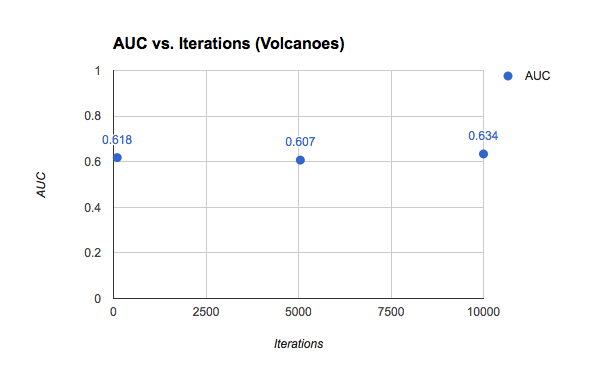
\includegraphics[width=\linewidth]{auc_iterations_volc.png}
      \caption{AUC vs Iterations for Volcanoes}
    \end{figure}
    \begin{figure}
      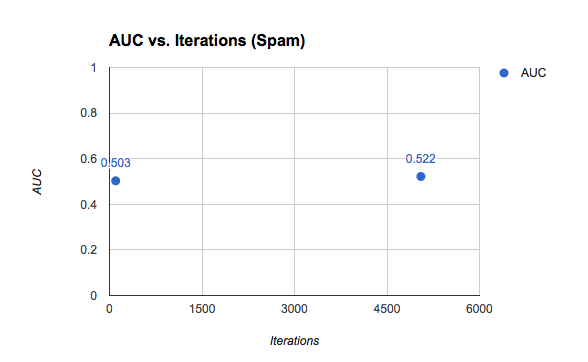
\includegraphics[width=\linewidth]{auc_iterations_spam.png}
      \caption{AUC vs Iterations for Spam}
    \end{figure}

    \begin{enumerate}
      \item Does the introduction of hidden units lead to improved accuracy?\\
        For volcanoes, yes, but only to a minor extent. While we don`t see the
        AUC improve when we add a hidden layer, the accuracy did improve from
        68\% in the perceptron to 70\% in the two layer ANN.\\
        For spam, there was no noticable improvement in accuracy.\\

      \item How many iterations does this ANN need to converge to compared to
        the perceptron?\\
        It took much longer for this ANN to converge. The perceptron from part
        a converged very quickly. This makes sense, since there are much fewer
        weights that need to be tuned.\\
    \end{enumerate}

  \item Explore how the AROC changes as the number of hidden units are varied
  on Voting and Volcanoes.\\
    \begin{figure}
      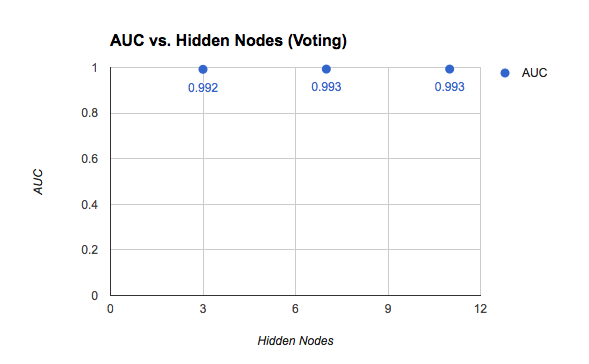
\includegraphics[width=\linewidth]{auc_nodes_vote.png}
      \caption{AUC vs Hidden Nodes for Voting}
    \end{figure}
    \begin{figure}
      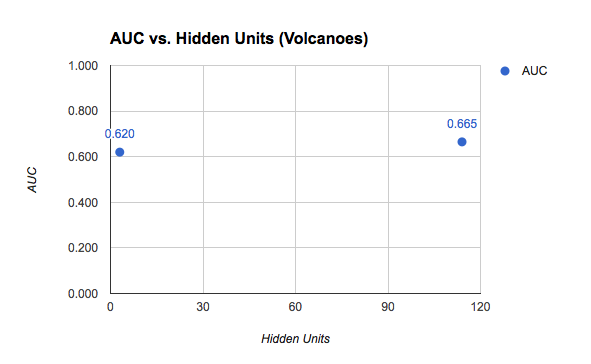
\includegraphics[width=\linewidth]{auc_nodes_volc.png}
      \caption{AUC vs Hidden Nodes for Volcanoes}
    \end{figure}
    For voting, ROC was marginally improved, going from approximately 0.98 to
    to 0.99. There was not much room from improvement here anyways, so it`s
    hard to say from just this example whether increasing the number of hidden
    nodes has any effect on the ROC. Training took a bit longer, due to the
    sheer number of iterations, but overall was not that bad, since voting is
    a rather small dataset.\\
    For volcanoes, ROC did not show much improvement if it all. Based on part
    b, it seems that increasing the number of training iterations has a greater
    effect on ROC than increasing the number of hidden nodes. Training took
    extremely long (several hours), likely due to the greater complexity of the
    volcanoes dataset relative to the voting dataset.

  \item Other observations:\\
    \begin{itemize}
      \item Training times were astronomically slower as the number of input
      units grew. Training spam was incredibly slower than voting, and even
      volcanoes.
      \item My ANN`s seemed to predict negative class labels much more often
      than positive. I am not entirely sure on why this would happen, but it
      certainly helped my precision scores.
      \item Implementing parallelization helped tremendously. Being able to
      train and evaluate all k folds (bounded by the number of cores on the
      machine, of course) at once was amazingly helpful. I did run into some
      issues with Python 2 vs 3 compatibility when implementing the
      parallelization, as the multiprocessing module exposes a different (and
      much better, for what I wanted to do) interface, so I had to do some
      ugliness (noted in a nearby comment in the code) to get it to work on
      both versions. Unfortunately, I seem to have implemented my
      parallelization too late, and was not able to get all of the data for
      two of the plots.
    \end{itemize}
\end{enumerate}
\end{document}
